\chapter{Technology Review}
This section includes information on the technologies used in the project as well as reasons they were chosen. It also focuses on the benefits of each technology used and their role in the entire system.

\section{Technology Selection Overview}
When deciding technologies to use for this project, insurance that they were all suitable for the clients needs and that they could be used to create a system which was satisfactory to the client was critical. With this type of project there are many different stacks which can be used to carry out web application development. Rather than use traditional stacks such as MEAN (MongoBD, Express, Angular and Node), the decision was made to vary off using a custom stack of technologies which had not been used in the past or at least usage of technologies with which minimal experience was had as a challenge The stack used consists of React.js, Flask and MongoDB. \\ \\
Technology Implementation Breakdown:
\begin{itemize}
    \item Web Application Front End: React.js
    \item Backend Server: Flask
    \item Database Storage: MongoDB
    \item Cloud: Heroku
\end{itemize}
\newpage

\section{ReactJS}
React is a Javascript Library which is used for building user interfaces. It was originally developed by Facebook. Due to react being a library, It allows for the plugin of many additional libraries to handle specific tasks e.g. routing and state management. React itself is only concerned with rendering document object model (DOM) data. Being a library means developers are not held down to a framework and allows for quick learning time meaning development can be started sooner. \par
React is component based which allows for splitting of UI into independant, reusable sections that manage their own state. React also uses a virtual DOM which creates an in memory cache for data structures, checks differences and then updates the displayed DOM efficiently \cite{10.1145/2980991}. This enables a programmer to develop as though the entire page is rendered with every change.
\begin{figure}[h!]
 	\caption{Example of a basic React component}
	\label{image:reactcomponent}
 	\centering
 	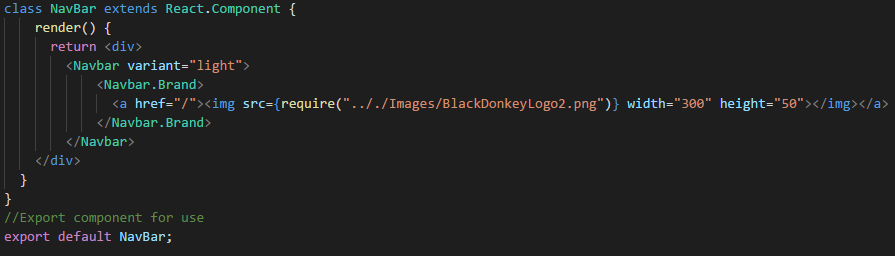
\includegraphics[width=1.0\textwidth]{Images/reactcomponent.PNG}
\end{figure}

\subsection{JavaScript XML (JSX)}
JSX is an extension of the JavaScript language. Although not necessary for React to write components, it is the generally recommended way for component creation. It allows developers to write HTML(Hypertext Markup Language) code in a way that is representative of XML format. JSX allows the HTML and JS to be linked directly. This allows for the user to easily interact and combine both e.g. render lists of data.

\begin{figure}[h!]
 	\caption{Example of JSX mapping a list}
	\label{image:jsx}
 	\centering
 	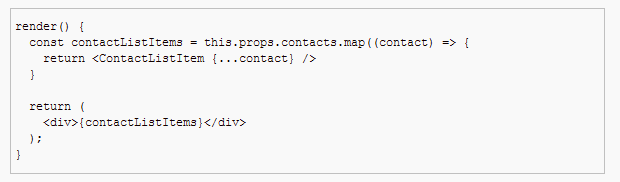
\includegraphics[width=0.9\textwidth]{Images/JSX Example.PNG}
\end{figure}

\subsection{React Hooks}
React Hooks are a way for the developer to manage and change React state and lifecycle. This allows developers to do so without the use of a class. There are many built in hooks within React with the most used being useEffect and useState. The useState hook is used for controlling the state, they allow for updating of state using the previous value and use a function to update it. While useEffect on the other hand is used for running your “effect” after flushing changes to the DOM \cite{tran2020tooling}. Effects must be declared inside the component so they have access to its props and state.

\section{Flask}
Flask is a lightweight web server gateway interface (WSGI) web application framework. Flask does not require any dependencies meaning it is a simplistic and flexible bare-minimum web server, and hence is promoted as a micro-framework \cite{vogel2017low}. This allows the developer to select the tools and libraries they wish to incorporate.
\begin{figure}[h!]
 	\caption{Basic implementation of a Flask server}
	\label{image:flask}
 	\centering
 	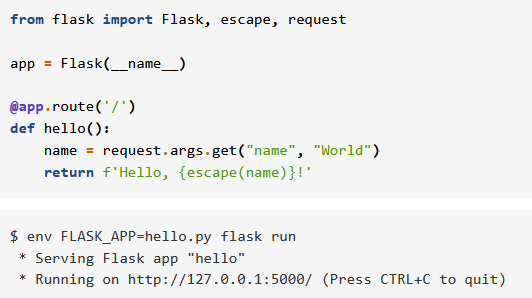
\includegraphics[width=0.9\textwidth]{Images/flask.PNG}
\end{figure}
\newpage

\subsection{Flask Blueprints}
Flask uses blueprints for adding components within a Flask application. They also allow support of common patterns from within an application or across applications. They simplify an application and provide Flask a way of adding extensions to register components on an application \cite{stouffer2015mastering}. In simplistic terms, a blueprint is not an application but a method to extend an application. In the application blueprints are used to extend API routes onto the Flask application itself.

\section{MongoDB}
The database used in this project is MongoDB. It is an open source NoSQL database. It uses a document based model to store data. The document data is stored in BSON, a binary encoding of JSON. It uses key-value pairs to store the data. MongoDB stores these documents in separate collections. These are alternatives to tables and rows in relational databases. A database may contain many collections each filled with many documents. The collections don’t have a fixed structure and fields can be of different data types \cite{boicea2012mongodb}.
\begin{figure}[h!]
 	\caption{Breakdown of MongoDB vs a Relational Database}
	\label{image:mongo}
 	\centering
 	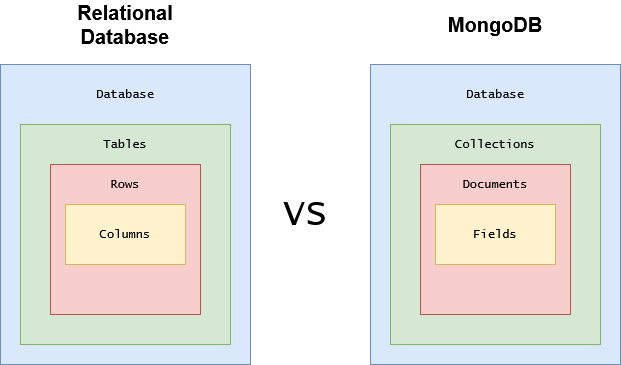
\includegraphics[width=0.9\textwidth]{Images/mongodb vs rdbms.png}
\end{figure}
\newpage

\subsection{PyMongo}
PyMongo is a Python distribution containing tools for working with MongoDB \cite{pedersen2014mining}. It allows a developer to connect a Python application to a MongoDB database. Pymongo handles querying of the database, as well as inserting, updating and deleting collections. PyMongo allows for rapid data transfer to and from the database allowing for seamless data access.
\begin{figure}[h!]
 	\caption{Sample of basic PyMongo connection and query}
	\label{image:pymongo}
 	\centering
 	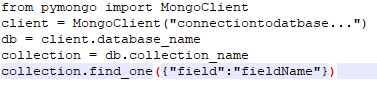
\includegraphics[width=0.75\textwidth]{Images/pymongosample.PNG}
\end{figure}
\newpage

\section{JSON (JavaScript Object Notation)}
JavaScript Object Notation, also known as JSON is a lightweight data-interchange format. It is a text based language so it is not only readable by machine, but also to humans. This makes it easy for humans to both read and write JSON \cite{nurseitov2009comparison}. Due to its lightweight nature JSON is easily parsed and generated by machines. JSON is also language independent so it can be used in a wide variety of programming languages and due to its popularity it is widely supported. JSON stores values using key-value pairs and supports many data types including strings, numbers, objects, arrays and boolean values etc.\par
JSON is used in many databases as a method of storage due to its rapid storage and retrieval capabilities. Using JSON allows databases not to have to worry about data manipulation. 
\begin{figure}[h!]
 	\caption{Example of JSON syntax}
	\label{image:JSON}
 	\centering
 	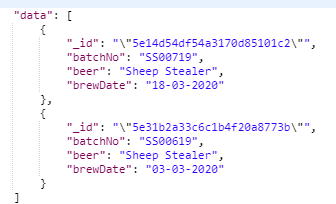
\includegraphics[width=0.9\textwidth]{Images/json example.PNG}
\end{figure}
\newpage

\section{Hypertext Transfer Protocol (HTTP)}
 Hypertext Transfer Protocol is an application-level protocol for distributed, collaborative, hypermedia information systems. HTTP allows for the transfer of files, for example images, text, videos etc across the world wide web. HTTP uses a set of methods to determine what it wants in a request. \\ \\
The methods used by HTTP include \cite{fielding1999hypertext}:
\begin{itemize}
    \item GET
    \item POST
    \item PUT
    \item DELETE
    \item PATCH
    \item HEAD
    \item OPTIONS
    \item CONNECT
    \item TRACE
\end{itemize}

\section{Representational State Transfer (REST)}
Representational State Transfer or more commonly known as REST is a software architectural style that outlines a set of constraints to be used for creating web services. REST is a method of implementation of HTTP methods. Similar to HTTP, REST uses GET, POST, PUT and DELETE and so on. This ensures applications can use the same methods of communication used on the internet. REST is stateless, therefore does not store any state about the client session on the server side. This allows the server not to have to deal with storing information about requests made, leading to faster responses \cite{khare2004extending}. REST being a web based architecture, allows for a response to be cached to improve performance.

\section{Testing Technology}
This section details a brief look at some of the technology which was used during the testing process.

\subsection{PyTest}
PyTest is a python framework that is used in order to carry out testing within python applications and files. PyTest is a command-line tool that automatically finds tests in your code, runs the tests, and gives a description of the results.\cite{okken2017python} It can be extended by writing plugins or installing third-party plugins. This was used for testing the calculations necessary on all data processed in the API server. This gave assurance that all calculations were correct which allowed progress on other areas of the project to continue development. These automated tests also ensured that new changes didn’t affect the calculations.
\begin{figure}[h!]
 	\caption{Sample of basic implementation of PyTest}
	\label{image:pytestimpl}
 	\centering
 	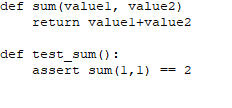
\includegraphics[width=0.5\textwidth]{Images/pytestsample.PNG}
\end{figure}

\subsection{Postman}
Postman is a collaboration platform for API development. HTTP requests can be made through Postman \cite{soniapi}. Postman's features simplify each step of building an API and streamline collaboration so you can create better and more efficient APIs. Postman was used extensively to test the API server and ensure that all aspects of the API functioned correctly and performed to a high standard.

\subsection{Selenium}
Selenium is a framework which is used to test web applications functionality. It uses simple scripts to run tests directly within a browser. It carries out these tests by embedding the automation into the browser \cite{holmes2006automating}. This was used by creating test cases for parts of the web application to guarantee their functionality was correct. This allowed retesting of older functioning components to check new integrations didn't break the previously passing tests.

\section{Security Technology}
This section discusses some of the technology which was used to ensure security precautions and measures were included in the project

\subsection{JSON web tokens (JWT)}
JSON Web Tokens are an open, industry standard method for representing claims securely between two parties. A web token is generally issued by a secure identity provider and used by a separate party that relies on its content to identify the token's subject for security-related purposes \cite{jones2015json}. This allows a logged in, verified user to send their web token with a request to authorize the return of data from the API server.
\newpage
\subsection{Okta}
Okta provides secure identity management with Single Sign-On and Multi-factor Authentication to ensure that the user is authorized to access data in the web application. The application must be registered on Okta provided developer console and Okta user accounts must be given access in order to log in to the specified site. This allows for user and password protection to be handled external to the web application.
\begin{figure}[h!]
 	\caption{Example of Okta single sign-on}
	\label{image:okta}
 	\centering
 	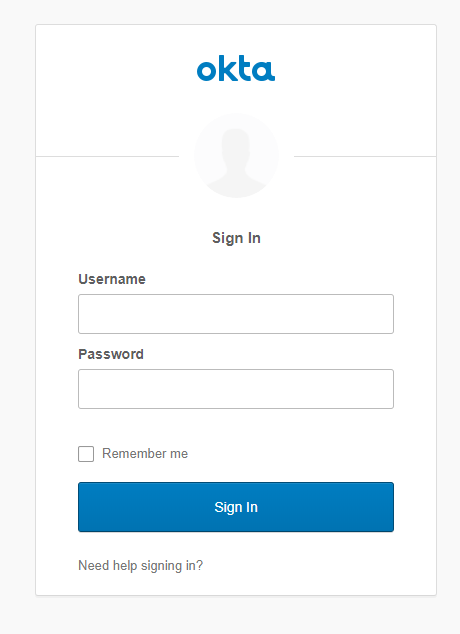
\includegraphics[width=0.75\textwidth]{Images/okta.PNG}
\end{figure}
\newpage
\section{Heroku}
Heroku is a platform as a service (PaaS) that enables developers to build, run, and operate applications entirely in the cloud. This allows for the hosting of the web application and server and allows for communication between them. It also allows for communication to the database from the server. This allows access to the application from anywhere in the world provided the user has an internet application which allows for universal usage of the application as it is not tied down to installation on a device. 

\section{Github}
Github is a company that provides hosting for software development version control using Git. It was used throughout development as a version control for the project. This was integral as it allowed a backup system for all coding done on the project as well as providing a means to record workflow of the project. This helped ensure progress of the project was on schedule and gave an account of each piece of work carried out in a sprint cycle.